\pdfminorversion=4
\documentclass[aspectratio=169]{beamer}

\mode<presentation>
{
  \usetheme{default}
  \usecolortheme{default}
  \usefonttheme{default}
  \setbeamertemplate{navigation symbols}{}
  \setbeamertemplate{caption}[numbered]
  \setbeamertemplate{footline}[frame number]  % or "page number"
  \setbeamercolor{frametitle}{fg=white}
  \setbeamercolor{footline}{fg=black}
} 

\usepackage[english]{babel}
\usepackage[utf8x]{inputenc}
\usepackage{tikz}
\usepackage{courier}
\usepackage{array}
\usepackage{bold-extra}
\usepackage{minted}
\usepackage[thicklines]{cancel}
\usepackage{fancyvrb}

\xdefinecolor{dianablue}{rgb}{0.18,0.24,0.31}
\xdefinecolor{darkblue}{rgb}{0.1,0.1,0.7}
\xdefinecolor{darkgreen}{rgb}{0,0.5,0}
\xdefinecolor{darkgrey}{rgb}{0.35,0.35,0.35}
\xdefinecolor{darkorange}{rgb}{0.8,0.5,0}
\xdefinecolor{darkorange2}{rgb}{1,0.5,0}
\xdefinecolor{darkred}{rgb}{0.7,0,0}
\xdefinecolor{darkpink}{rgb}{0.9,0.2,0.6}
\definecolor{darkgreen}{rgb}{0,0.6,0}
\definecolor{mauve}{rgb}{0.58,0,0.82}

\title[2019-03-14-awkward-acat2019]{Nested data structures in array and SIMD frameworks}
\author{Jim Pivarski}
\institute{Princeton University -- DIANA-HEP, IRIS-HEP}
\date{March 14, 2019}

\usetikzlibrary{shapes.callouts}

\begin{document}

\logo{\pgfputat{\pgfxy(0.11, 7.4)}{\pgfbox[right,base]{\tikz{\filldraw[fill=dianablue, draw=none] (0 cm, 0 cm) rectangle (50 cm, 1 cm);}\mbox{\hspace{-8 cm}
\includegraphics[height=1 cm]{princeton-logo-long.png}
\includegraphics[height=1 cm]{diana-hep-logo-long.png}}}}}

\begin{frame}
  \titlepage
\end{frame}

\logo{\pgfputat{\pgfxy(0.11, 7.4)}{\pgfbox[right,base]{\tikz{\filldraw[fill=dianablue, draw=none] (0 cm, 0 cm) rectangle (50 cm, 1 cm);}\mbox{\hspace{-8 cm}
\includegraphics[height=1 cm]{princeton-logo.png}
\includegraphics[height=1 cm]{diana-hep-logo.png}}}}}

% Uncomment these lines for an automatically generated outline.
%\begin{frame}{Outline}
%  \tableofcontents
%\end{frame}

% START START START START START START START START START START START START START

%% \begin{frame}[fragile]{Nested, variable-sized data structures are crucial in HEP}
%% \vspace{0.5 cm}
%% \begin{columns}
%% \column{0.5\linewidth}
%% 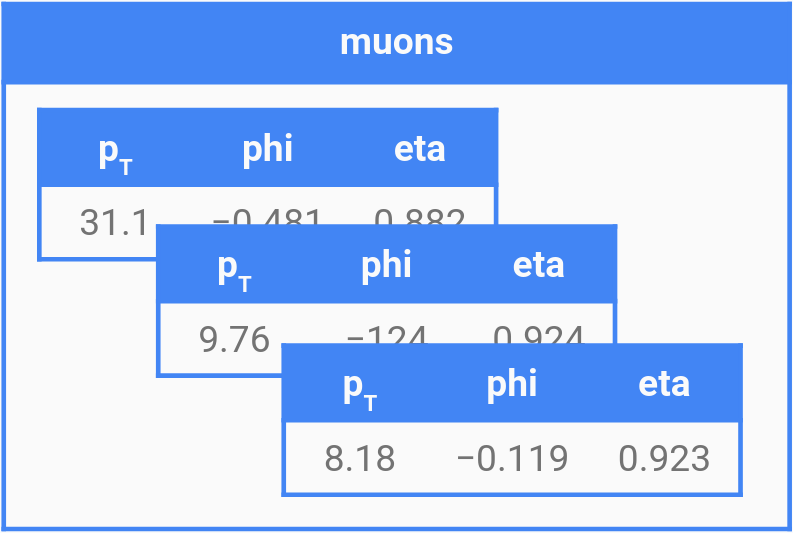
\includegraphics[width=\linewidth]{muons-as-objects.png}

%% \column{0.5\linewidth}
%% 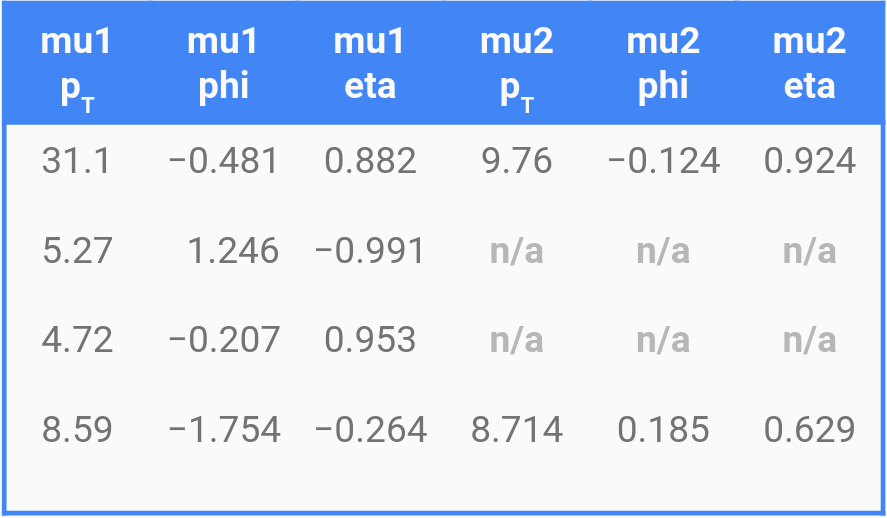
\includegraphics[width=\linewidth]{muons-as-a-table.png}
%% \end{columns}

%% \begin{uncoverenv}<2>
%% \vspace{0.4 cm}
%% Most of our analysis data are big lists of variable-length lists of structs/objects/records.

%% \vspace{0.25 cm}
%% \scriptsize
%% \begin{Verbatim}[commandchars=\\\{\}]
%% [[Muon(\textcolor{darkgreen}{31.1}, \textcolor{darkorange}{-0.481}, \textcolor{blue}{0.882}), Muon(\textcolor{darkgreen}{9.76}, \textcolor{darkorange}{-0.124}, \textcolor{blue}{0.924}), Muon(\textcolor{darkgreen}{8.18}, \textcolor{darkorange}{-0.119}, \textcolor{blue}{0.923})],
%%  [Muon(\textcolor{darkgreen}{5.27}, \textcolor{darkorange}{1.246}, \textcolor{blue}{-0.991})],
%%  [Muon(\textcolor{darkgreen}{4.72}, \textcolor{darkorange}{-0.207}, \textcolor{blue}{0.953})],
%%  [Muon(\textcolor{darkgreen}{8.59}, \textcolor{darkorange}{-1.754}, \textcolor{blue}{-0.264}), Muon(\textcolor{darkgreen}{8.714}, \textcolor{darkorange}{0.185}, \textcolor{blue}{0.629})],
%%  ...
%% \end{Verbatim}
%% \end{uncoverenv}
%% \end{frame}

%% \begin{frame}[fragile]{Columnar representation}
%% \vspace{0.5 cm}

%% But they don't have to be ``structs,'' pointers to contiguous $p_T$, $\eta$, $\phi$ triples.

%% \scriptsize
%% \begin{Verbatim}[commandchars=\\\{\}]
%% [[Muon(\textcolor{darkgreen}{31.1}, \textcolor{darkorange}{-0.481}, \textcolor{blue}{0.882}), Muon(\textcolor{darkgreen}{9.76}, \textcolor{darkorange}{-0.124}, \textcolor{blue}{0.924}), Muon(\textcolor{darkgreen}{8.18}, \textcolor{darkorange}{-0.119}, \textcolor{blue}{0.923})],
%%  [Muon(\textcolor{darkgreen}{5.27}, \textcolor{darkorange}{1.246}, \textcolor{blue}{-0.991})],
%%  [Muon(\textcolor{darkgreen}{4.72}, \textcolor{darkorange}{-0.207}, \textcolor{blue}{0.953})],
%%  [Muon(\textcolor{darkgreen}{8.59}, \textcolor{darkorange}{-1.754}, \textcolor{blue}{-0.264}), Muon(\textcolor{darkgreen}{8.714}, \textcolor{darkorange}{0.185}, \textcolor{blue}{0.629})],
%%  ...
%% \end{Verbatim}
%% \normalsize

%% \vspace{0.5 cm}
%% They can be contiguous by field with offsets or starts/stops or counts or parents or\ldots

%% \vspace{0.25 cm}
%% \begin{tabular}{r l}
%% \only<1>{\small offsets &                    {\tt\scriptsize \ \ \ \ \ 0,\ \ \ \ \ \ \ \ \ \ \ \ \ \ \ \ \ \ \ \ \ \ 3,\ \ \ \ \ \ 4,\ \ \ \ \ \ 5,\ \ \ \ \ \ \ 7} \\}
%% \only<3>{\small parents &                    {\tt\scriptsize \ \ \ \ \ 0,\ \ \ \ \ \ 0,\ \ \ \ \ \ 0,\ \ \ \ \ \ 1,\ \ \ \ \ \ 2,\ \ \ \ \ \ 3,\ \ \ \ \ 3} \\}
%% \only<2>{\small starts  &                    {\tt\scriptsize \ \ \ \ \ 0,\ \ \ \ \ \ \ \ \ \ \ \ \ \ \ \ \ \ \ \ \ \ 3,\ \ \ \ \ \ 4,\ \ \ \ \ \ 5\ \ \ \ \ \ \ \ \ } \\}
%% \uncover<2>{\small stops   &                    {\tt\scriptsize \ \ \ \ \ 3,\ \ \ \ \ \ \ \ \ \ \ \ \ \ \ \ \ \ \ \ \ \ 4,\ \ \ \ \ \ 5,\ \ \ \ \ \ 7\ \ \ \ \ \ \ \ \ } \\}
%% \small $p_T$ & \textcolor{darkgreen}{\tt\scriptsize \ \ 31.1,\ \ \ 9.76,\ \ \ 8.18,\ \ \ 5.27,\ \ \ 4.72,\ \ \ 8.59, 8.714} \\
%% \small phi &  \textcolor{darkorange}{\tt\scriptsize -0.481,\ -0.123,\ -0.119,\ \ 1.246,\ -0.207,\ -1.754,\ 0.185} \\
%% \small eta &        \textcolor{blue}{\tt\scriptsize \ 0.882,\ \ 0.924,\ \ 0.923,\ -0.991,\ \ 0.953,\ -0.264,\ 0.629} \\
%% \end{tabular}
%% \end{frame}

%% \begin{frame}[fragile]{This allows for efficient ways of {\it manipulating} data}
%% \vspace{0.25 cm}

%% ``Remove the first muon from each event.'' \uncover<2->{\textcolor{red}{$\longrightarrow$ rewrite all inner lists.}}

%% \scriptsize
%% \begin{onlyenv}<1>
%% \begin{Verbatim}[commandchars=\\\{\}]
%% [[Muon(\textcolor{darkgreen}{31.1}, \textcolor{darkorange}{-0.481}, \textcolor{blue}{0.882}), Muon(\textcolor{darkgreen}{9.76}, \textcolor{darkorange}{-0.124}, \textcolor{blue}{0.924}), Muon(\textcolor{darkgreen}{8.18}, \textcolor{darkorange}{-0.119}, \textcolor{blue}{0.923})],
%%  [Muon(\textcolor{darkgreen}{5.27}, \textcolor{darkorange}{1.246}, \textcolor{blue}{-0.991})],
%%  [Muon(\textcolor{darkgreen}{4.72}, \textcolor{darkorange}{-0.207}, \textcolor{blue}{0.953})],
%%  [Muon(\textcolor{darkgreen}{8.59}, \textcolor{darkorange}{-1.754}, \textcolor{blue}{-0.264}), Muon(\textcolor{darkgreen}{8.714}, \textcolor{darkorange}{0.185}, \textcolor{blue}{0.629})],
%%  ...
%% \end{Verbatim}
%% \end{onlyenv}\begin{onlyenv}<2->
%% \begin{Verbatim}[commandchars=\\\{\}]
%% [[     \textcolor{darkgreen}{    }  \textcolor{darkorange}{      }  \textcolor{blue}{     }   Muon(\textcolor{darkgreen}{9.76}, \textcolor{darkorange}{-0.124}, \textcolor{blue}{0.924}), Muon(\textcolor{darkgreen}{8.18}, \textcolor{darkorange}{-0.119}, \textcolor{blue}{0.923})],
%%  [     \textcolor{darkgreen}{    }  \textcolor{darkorange}{     }  \textcolor{blue}{      } ],
%%  [     \textcolor{darkgreen}{    }  \textcolor{darkorange}{      }  \textcolor{blue}{     } ],
%%  [     \textcolor{darkgreen}{    }  \textcolor{darkorange}{      }  \textcolor{blue}{      }   Muon(\textcolor{darkgreen}{8.714}, \textcolor{darkorange}{0.185}, \textcolor{blue}{0.629})],
%%  ...
%% \end{Verbatim}
%% \end{onlyenv}
%% \normalsize

%% \vspace{0.5 cm}
%% ``Remove the first muon from each event.'' \uncover<2->{\textcolor{red}{$\longrightarrow$ increase all starts by 1.}}

%% \vspace{0.25 cm}
%% \begin{onlyenv}<1>
%% \begin{tabular}{r l}
%% \small starts  &                    {\tt\scriptsize \ \ \ \ \ 0,\ \ \ \ \ \ \ \ \ \ \ \ \ \ \ \ \ \ \ \ \ \ 3,\ \ \ \ \ \ 4,\ \ \ \ \ \ 5\ \ \ \ \ \ \ \ \ } \\
%% \small stops   &                    {\tt\scriptsize \ \ \ \ \ 3,\ \ \ \ \ \ \ \ \ \ \ \ \ \ \ \ \ \ \ \ \ \ 4,\ \ \ \ \ \ 5,\ \ \ \ \ \ 7\ \ \ \ \ \ \ \ \ } \\
%% \small $p_T$ & \textcolor{darkgreen}{\tt\scriptsize \ \ 31.1,\ \ \ 9.76,\ \ \ 8.18,\ \ \ 5.27,\ \ \ 4.72,\ \ \ 8.59, 8.714} \\
%% \small phi &  \textcolor{darkorange}{\tt\scriptsize -0.481,\ -0.123,\ -0.119,\ \ 1.246,\ -0.207,\ -1.754,\ 0.185} \\
%% \small eta &        \textcolor{blue}{\tt\scriptsize \ 0.882,\ \ 0.924,\ \ 0.923,\ -0.991,\ \ 0.953,\ -0.264,\ 0.629} \\
%% \end{tabular}
%% \end{onlyenv}\begin{onlyenv}<2->
%% \begin{tabular}{r l}
%% \small starts  &     \textcolor{red}{\tt\scriptsize \ \ \ \ \ 1,\ \ \ \ \ \ \ \ \ \ \ \ \ \ \ \ \ \ \ \ \ \ 4,\ \ \ \ \ \ 5,\ \ \ \ \ \ 6\ \ \ \ \ \ \ \ \ } \\
%% \small stops   &                    {\tt\scriptsize \ \ \ \ \ 3,\ \ \ \ \ \ \ \ \ \ \ \ \ \ \ \ \ \ \ \ \ \ 4,\ \ \ \ \ \ 5,\ \ \ \ \ \ 7\ \ \ \ \ \ \ \ \ } \\
%% \small $p_T$ & \textcolor{darkgreen}{\tt\scriptsize \ \ 31.1,\ \ \ 9.76,\ \ \ 8.18,\ \ \ 5.27,\ \ \ 4.72,\ \ \ 8.59, 8.714} \\
%% \small phi &  \textcolor{darkorange}{\tt\scriptsize -0.481,\ -0.123,\ -0.119,\ \ 1.246,\ -0.207,\ -1.754,\ 0.185} \\
%% \small eta &        \textcolor{blue}{\tt\scriptsize \ 0.882,\ \ 0.924,\ \ 0.923,\ -0.991,\ \ 0.953,\ -0.264,\ 0.629} \\
%% \end{tabular}\end{onlyenv}

%% \vspace{0.5 cm}
%% \uncover<3>{We didn't need to touch any contents (read them from disk, decompress them\ldots).}
%% \end{frame}

%% \begin{frame}{Library for manipulating non-standard array types}
%% \vspace{0.5 cm}
%% \begin{columns}
%% \column{0.45\linewidth}
%% 
\includegraphics[width=\linewidth]{awkward-logo.pdf}

%% \vspace{0.25 cm}
%% \hfill \scriptsize \textcolor{darkblue}{\url{github.com/scikit-hep/awkward-array}}

%% \column{0.55\linewidth}
%% \vspace{0.5 cm}
%% \vspace{2\baselineskip}
%% \begin{itemize}
%% \item variable-length subarrays
%% \item struct-of-arrays looking like array-of-structs
%% \item nullable types
%% \item heterogeneous types (tagged unions)
%% \item cross-references or even cyclic references
%% \item sparse, non-contiguous, lazy
%% \end{itemize}

%% \vspace{0.5 cm}
%% \uncover<2>{Any awkward array can be placed within any other awkward array.}
%% \end{columns}
%% \end{frame}

%% \begin{frame}[fragile]{Not lacking for data types}
%% \vspace{0.5 cm}
%% Nullable, heterogeneous, multiple levels of depth, nested records\ldots

%% \small
%% \begin{minted}{python}
%% >>> import awkward
%% >>> array = awkward.fromiter(
%% ...     [[1.1, 2.2, None, 3.3, None],
%% ...      [4.4, [5.5]],
%% ...      [{"x": 6, "y": {"z": 7}}, None, {"x": 8, "y": {"z": 9}}]])
%% \end{minted}

%% \begin{uncoverenv}<2->
%% \begin{minted}{python}
%% >>> print(array)            # internally, these are all arrays
%% [[1.1 2.2 None 3.3 None] [4.4 [5.5]] [<Row 0> None <Row 1>]]
%% \end{minted}
%% \end{uncoverenv}

%% \begin{uncoverenv}<3->
%% \begin{minted}{python}
%% >>> print(array[:, -2:])    # for all outer list, last two of inner
%% [[3.3 None] [4.4 [5.5]] [None <Row 1>]]
%% \end{minted}
%% \end{uncoverenv}

%% \begin{uncoverenv}<4->
%% \begin{minted}{python}
%% >>> (array + 100).tolist()  # element-wise function applied to arrays
%% [[101.1, 102.2, None, 103.3, None],
%%  [104.4, [105.5]],
%%  [{'x': 106, 'y': {'z': 107}}, None, {'x': 108, 'y': {'z': 109}}]]
%% \end{minted}
%% \end{uncoverenv}
%% \end{frame}

%% \begin{frame}{Columnar data structures minimize memory use and time}
%% \vspace{0.5 cm}
%% One operation, deriving $p_z$ of a variable number of $p_T$ and $\eta$ per event, using \textcolor{darkorange2}{awkward-array}, \textcolor{blue}{ROOT}, \textcolor{darkpink}{pure Python}, and \textcolor{darkgreen}{root\_numpy}.

%% \vspace{0.2 cm}
%% \begin{center}
%% 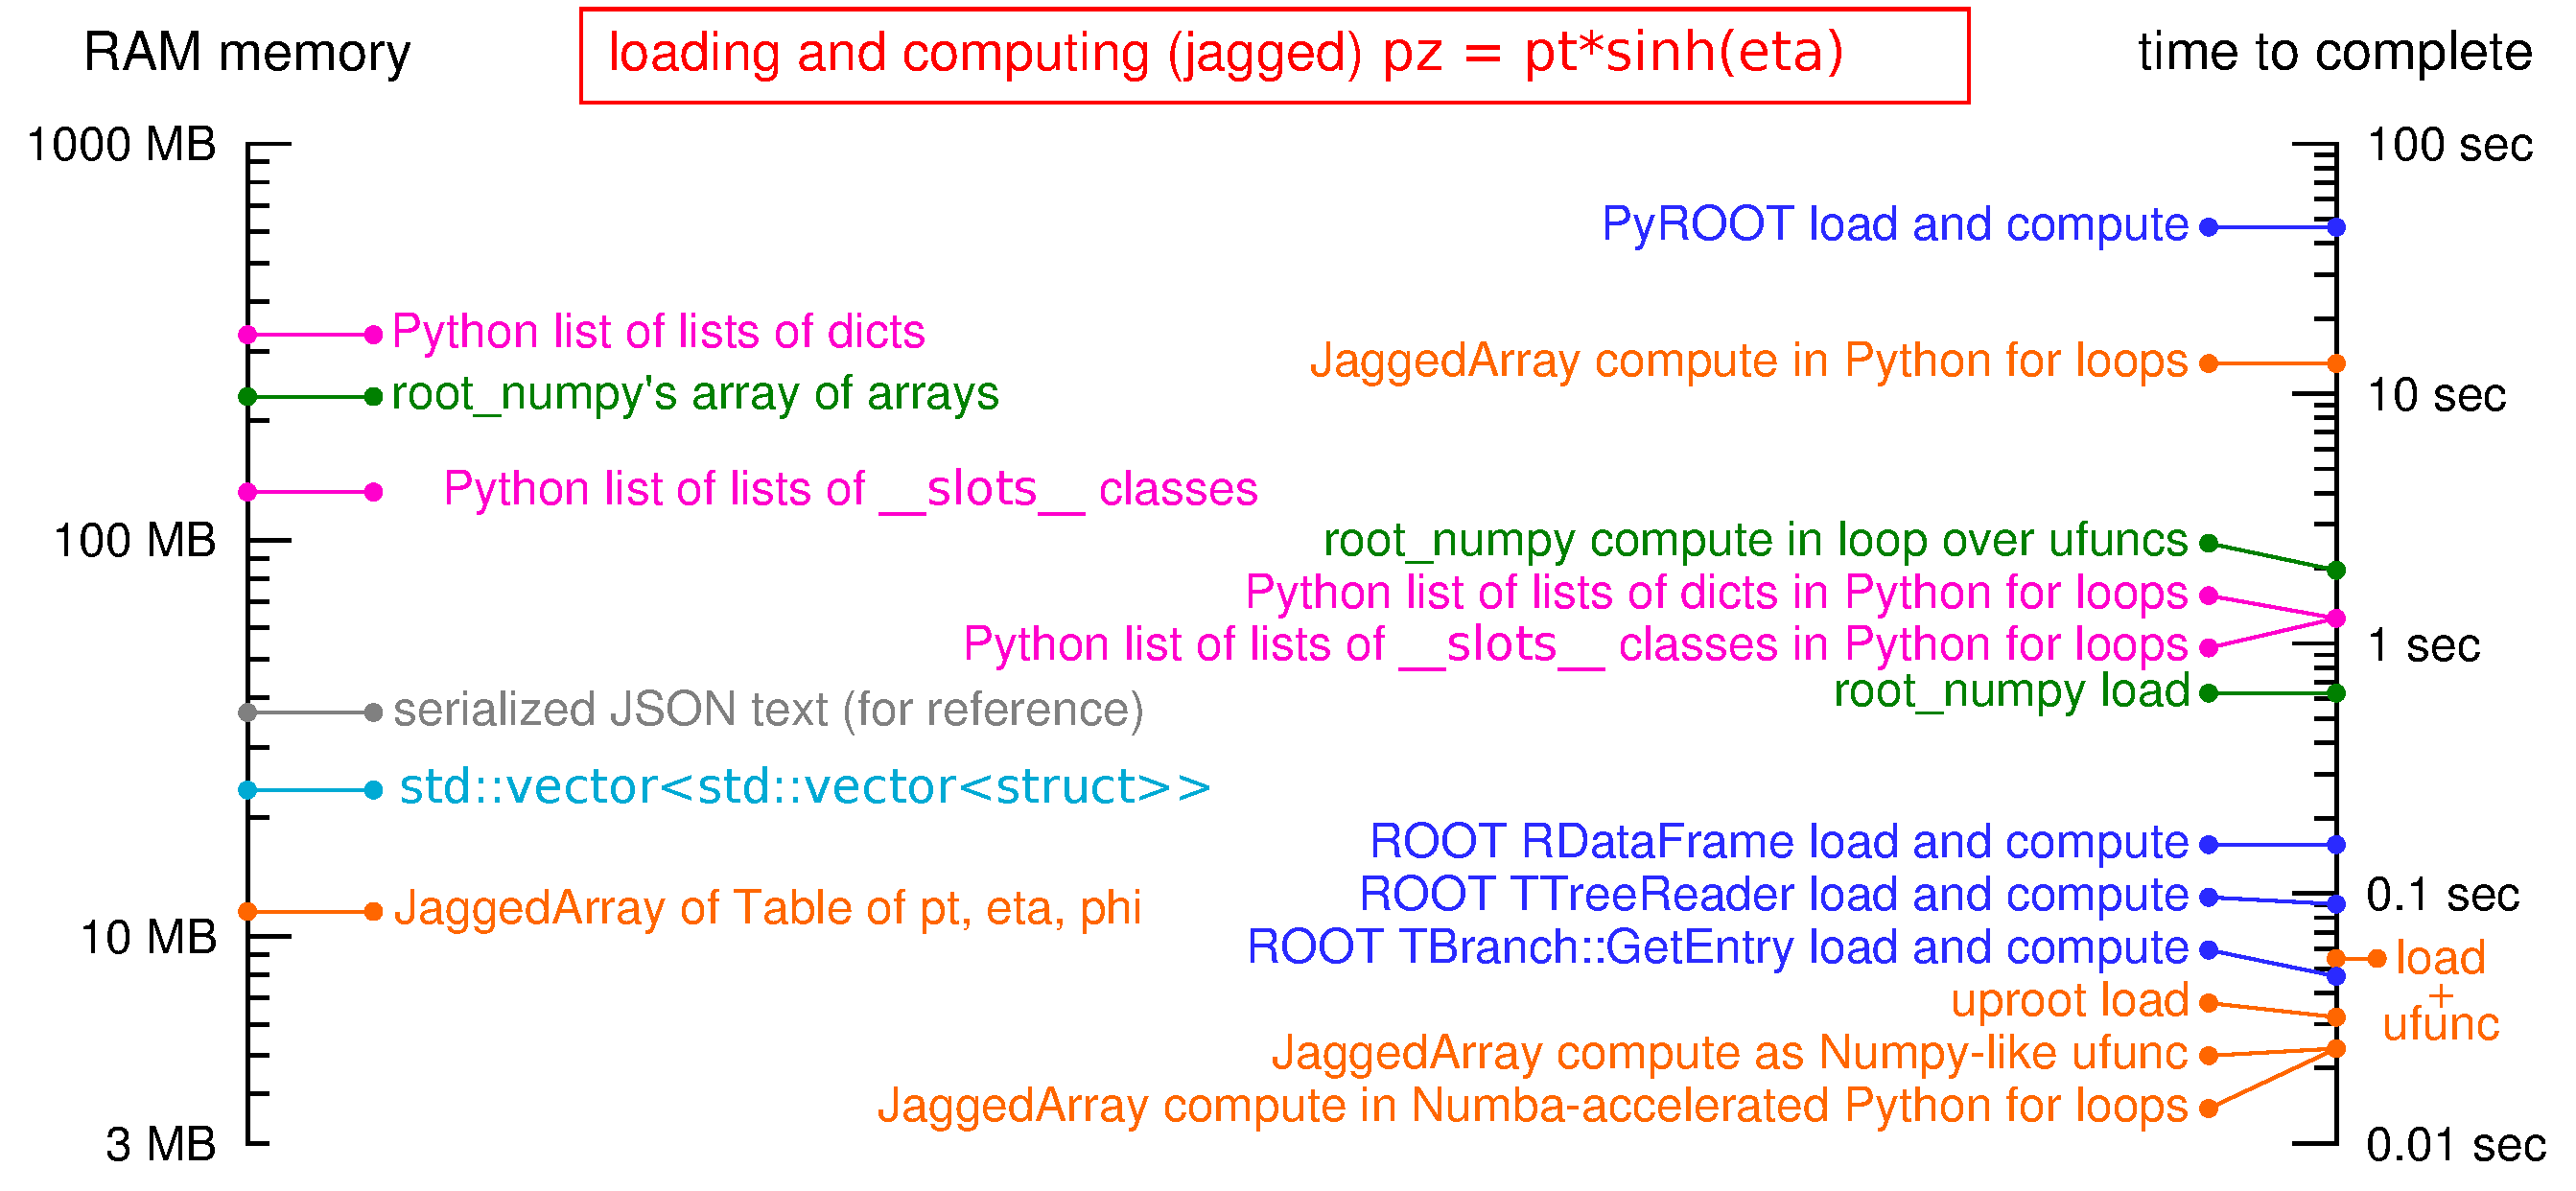
\includegraphics[width=0.9\linewidth]{logscales.pdf}
%% \end{center}
%% \end{frame}

%% \begin{frame}{Real life}
%% \vspace{0.5 cm}
%% \LARGE
%% \begin{center}
%% a single operation $\ne$ a physics analysis
%% \end{center}
%% \end{frame}

\begin{frame}{Real analyses using columnar tools}
\vspace{0.75 cm}
\begin{columns}
\column{0.2\linewidth}

\includegraphics[width=\linewidth]{coffea-logo.png}

\column{0.8\linewidth}
\hspace{-0.2 cm}\Huge Coffea

\vspace{0.25 cm}
\large {\bf C}olumnar {\bf O}bject {\bf F}ramework {\bf F}or {\bf E}fficient {\bf A}nalysis

\vspace{0.25 cm}
\normalsize Matteo~Cremonesi, Lindsey~Gray, Oliver~Gutsche, Allison~Hall, Bo~Jayatilaka, Igor~Mandrichenko, Kevin~Pedro, Nick~Smith~[FNAL], and~me~[Princeton] \hfill \textcolor{blue}{\url{github.com/CoffeaTeam}}
\end{columns}

\vspace{0.25 cm}
\begin{center}
\begin{minipage}{0.65\linewidth}
\Large Performing two complete CMS analyses:
\begin{itemize}
\item Dark Higgs search
\item Boosted SM $H \to b\bar{b}$
\end{itemize}
\end{minipage}
\end{center}
\end{frame}




\end{document}
